\documentclass{article}
%\usepackage{enumitem}
\usepackage[table]{xcolor}
\usepackage{listings}
\usepackage{amsfonts}
\usepackage{latexsym}
\usepackage{fullpage}
\usepackage{graphicx}
%\usepackage{paralist}
\usepackage{tikz-timing}
\usepackage{tabto}
\usepackage[utf8]{inputenc}
\usepackage[T1]{fontenc}
\usepackage{filecontents}
\usepackage[backend=biber,style=ieee]{biblatex}
\usepackage{caption}
\usepackage{subcaption}
\usepackage[brazilian]{babel}
\lstset{language=C}

\graphicspath{{images/}}

% Default margins are too wide all the way around. I reset them here
\setlength{\topmargin}{-.5in}
\setlength{\textheight}{9in}
\setlength{\oddsidemargin}{.125in}
\setlength{\textwidth}{6.25in}

\lstset{literate=
  {á}{{\'a}}1 {é}{{\'e}}1 {í}{{\'i}}1 {ó}{{\'o}}1 {ú}{{\'u}}1
  {Á}{{\'A}}1 {É}{{\'E}}1 {Í}{{\'I}}1 {Ó}{{\'O}}1 {Ú}{{\'U}}1
  {à}{{\`a}}1 {è}{{\`e}}1 {ì}{{\`i}}1 {ò}{{\`o}}1 {ù}{{\`u}}1
  {À}{{\`A}}1 {È}{{\'E}}1 {Ì}{{\`I}}1 {Ò}{{\`O}}1 {Ù}{{\`U}}1
  {ä}{{\"a}}1 {ë}{{\"e}}1 {ï}{{\"i}}1 {ö}{{\"o}}1 {ü}{{\"u}}1
  {Ä}{{\"A}}1 {Ë}{{\"E}}1 {Ï}{{\"I}}1 {Ö}{{\"O}}1 {Ü}{{\"U}}1
  {â}{{\^a}}1 {ê}{{\^e}}1 {î}{{\^i}}1 {ô}{{\^o}}1 {û}{{\^u}}1
  {Â}{{\^A}}1 {Ê}{{\^E}}1 {Î}{{\^I}}1 {Ô}{{\^O}}1 {Û}{{\^U}}1
  {œ}{{\oe}}1 {Œ}{{\OE}}1 {æ}{{\ae}}1 {Æ}{{\AE}}1 {ß}{{\ss}}1
  {ű}{{\H{u}}}1 {Ű}{{\H{U}}}1 {ő}{{\H{o}}}1 {Ő}{{\H{O}}}1
  {ç}{{\c c}}1 {Ç}{{\c C}}1 {ø}{{\o}}1 {å}{{\r a}}1 {Å}{{\r A}}1
  {€}{{\euro}}1 {£}{{\pounds}}1 {«}{{\guillemotleft}}1
  {»}{{\guillemotright}}1 {ñ}{{\~n}}1 {Ñ}{{\~N}}1 {¿}{{?`}}1
  {ã}{{\~a}}1 {Ã}{{\~A}}1
}

\definecolor{backgroundColour}{rgb}{0.95,0.95,0.92}

\lstdefinestyle{CStyle}{
    backgroundcolor=\color{backgroundColour},   
    basicstyle=\footnotesize,
    breakatwhitespace=false,         
    breaklines=true,                 
    captionpos=b,                    
    keepspaces=true,                 
    numbers=left,                    
    numbersep=5pt,                  
    showspaces=false,                
    showstringspaces=false,
    showtabs=false,                  
    tabsize=2,
    language=C
}

\renewcommand{\lstlistingname}{Exemplo}

% Defining references here

\begin{filecontents}{\jobname.bib}
@article{singh2014,
author = {Dhananjay, Singh and Gaurav, Tripathi},
year = {2014},
month = {03},
pages = {},
title = {A Survey of Internet-of-Things: Future Vision, Architecture, Challenges and Services},
journaltitle = {2014 IEEE World Forum on Internet of Things, WF-IoT 2014}
}
@online{arduinoblog,
author = {Arduino},
title = {Arduino Blog},
year = {2017},
url = {https://blog.arduino.cc},
OPTnote = {Acessado em 24 de Abril de 2017}
}
@article{santanna2012,
author = {Francisco Sant’Anna and
Noemi de La Rocque Rodriguez and
Roberto Ierusalimschy},
title = {CÉU: Embedded, Safe, and
Reactive},
journaltitle = {Monografias em Ciência da Computação},
year = {2012},
volume = {9},
issn = {0103-9741}
}
@online{githubceuarduino,
author = {Francisco Sant'Anna},
title = {GitHub Céu-Arduino},
year = {2017},
url = {https://github.com/fsantanna/ceu-arduino},
note = {Acessado em 24 de Abril de 2017}
}
@article{wortmann2015,
author = {Felix Wortmann and Kristina Flütcher},
year = {2015},
pages = {221-224},
title = {Internet of Things - Technology and Value Added},
journaltitle = {Business \& Information Systems Engineering},
volume = {57},
issue = {3}
}
@periodical{chui2010,
editor = {Michael Chui and Markus Löffer and Roger Roberts},
title = {The Internet of Things},
year = {2010},
series = {McKinsey Quarterly},
month = {Março},
url = {https://www.mckinsey.com/industries/high-tech/our-insights/the-internet-of-things}
}
@ARTICLE{edwards1997, 
author={S. Edwards and L. Lavagno and E. A. Lee and A. Sangiovanni-Vincentelli}, 
journal={Proceedings of the IEEE}, 
title={Design of embedded systems: formal models, validation, and synthesis}, 
year={1997}, 
volume={85}, 
number={3}, 
pages={366-390}, 
keywords={application specific integrated circuits;computer architecture;formal specification;formal verification;logic design;real-time systems;systems analysis;ASIC;application-specific integrated circuits;concurrent design process;embedded software;embedded systems design;formal models;formal validation;heterogeneous systems;reactive real-time system design;specification;Application software;Application specific integrated circuits;Computer architecture;Consumer electronics;Embedded computing;Embedded system;Hardware;Microcontrollers;Real time systems;Safety}, 
doi={10.1109/5.558710}, 
ISSN={0018-9219}, 
month={Mar},}
@online{githubceu,
author = {Francisco Sant'Anna},
title = {GitHub Céu},
year = {2017},
url = {https://github.com/fsantanna/ceu},
note = {Acessado em 24 de Abril de 2017}
}
@manual{atmegadatasheet,
author = {AtMel},
title = {AtMel ATmega328/P DATASHEET},
year = {2016},
organization = {ATMel},
}

\end{filecontents}

\addbibresource{\jobname.bib}

% End defining references

\begin{document}

\begin{titlepage}

\newcommand{\HRule}{\rule{\linewidth}{0.5mm}} % Defines a new command for the horizontal lines, change thickness here

\center % Center everything on the page
 
%----------------------------------------------------------------------------------------
%	HEADING SECTIONS
%----------------------------------------------------------------------------------------

\textsc{\LARGE Pontifícia Universidade Católica do Rio de Janeiro}\\[1.5cm] % Name of your university/college
\textsc{\Large Projeto Final de Graduação de Engenharia da Computação}\\[0.5cm] % Minor heading such as course title

\textsc{\large Departamento de Informática - DI \\ Centro Técnico Científico - CTC \\ Curso de Engenharia da Computação}\\[0.5cm] % Major heading such as course name


%----------------------------------------------------------------------------------------
%	TITLE SECTION
%----------------------------------------------------------------------------------------

\HRule \\[0.4cm]
{ \huge \bfseries Aplicação em Sistemas Distribuídos
utilizando biblioteca e driver próprios,
baseados em interrupções desenvolvido
em Céu para o microcontrolador Arduino}\\[0.4cm] % Title of your document
\HRule \\[1.5cm]
 
%----------------------------------------------------------------------------------------
%	AUTHOR SECTION
%----------------------------------------------------------------------------------------

\begin{minipage}{0.4\textwidth}
\begin{flushleft} \large
\emph{Aluno:}\\
Guilherme \textsc{Simas} % Your name
\end{flushleft}
\end{minipage}
~
\begin{minipage}{0.4\textwidth}
\begin{flushright} \large
\emph{Orientador:} \\
Ana \textsc{Lúcia de Moura} % Supervisor's Name
\end{flushright}
\end{minipage}\\[4cm]

% If you don't want a supervisor, uncomment the two lines below and remove the section above
%\Large \emph{Author:}\\
%John \textsc{Smith}\\[3cm] % Your name

%----------------------------------------------------------------------------------------
%	DATE SECTION
%----------------------------------------------------------------------------------------

{\large \today}\\[3cm] % Date, change the \today to a set date if you want to be precise

%----------------------------------------------------------------------------------------
%	LOGO SECTION
%----------------------------------------------------------------------------------------

%\includegraphics{Logo}\\[1cm] % Include a department/university logo - this will require the graphicx package
 
%----------------------------------------------------------------------------------------

\vfill % Fill the rest of the page with whitespace

\end{titlepage}

\newpage % Dedicatória

\begin{flushright}

\vspace*{\fill}

\textit{\LARGE Agradecimentos estarão descritos nesse bloco de texto. Caso o bloco de texto seja grande demais espera-se que ele pule linhas e continue se guiando pela margem direita}

\vspace*{\fill}

\end{flushright}

\newpage

\tableofcontents{}

\newpage

\section{Introdução}	


\tab Existem várias definições do termo “Internet das
Coisas”, porém a grande maioria delas compartilha a ideia de que a conexão e troca de dados
entre elementos é parte vital do conceito. Por esse motivo, a área de Sistemas Distribuídos possui um
papel importantíssimo nesse desenvolvimento, já que toda aplicação deve ser capaz de trocar
mensagens e informação segura e corretamente de forma a se sincronizar, e de forma escalável. \cite{singh2014}
Outro ponto sobre a escalabilidade de aplicações em Internet das Coisas é a necessidade de unidades
computacionais de custo baixo e consumo eficiente de energia. Por esse motivo microcontroladores
são outra parte vital do desenvolvimento de soluções, apresentando, entre outras vantagens, uma
facilidade na programação devido a bibliotecas e drivers já implementados e disponibilizados.
Microcontroladores são capazes de processamento de dados por possuírem processadores e de
serem facilmente integrados com sensores e atuadores, possuindo hardware especializado para
interfacear com esses componentes.
\par Muitas ferramentas de desenvolvimento fornecidos para microcontroladores incluem rotinas que causam um bloqueio na
aplicação, ou seja, enquanto está realizando a chamada correspondente àquela funcionalidade, o
software entra em um estado onde realiza tarefas virtualmente inúteis até que o hardware conclua sua
parte. Esse comportamento é indesejável visto que a aplicação desperdiça tempo aguardando o
hardware enquanto poderia estar realizando outras tarefas como, por exemplo, um processamento de
dados recebidos por uma mensagem, ou a troca de mensagens em si. Essa ineficiência marca um
desperdício de tempo e consumo de energia.
\par O bloqueio de aplicações é um desafio enfrentado frequentemente em aplicações que envolvem
sistemas nos quais o tempo de processamento ou reação a estímulos externos é pertinente ao
funcionamento da aplicação. O paradigma de programação orientada a eventos é muitas vezes
utilizado como abordagem nessas situações. Em uma aplicação orientada a eventos, o sistema segue
seu fluxo normal até a chegada de um “evento”, como a chegada de uma mensagem, ou a conclusão
de um trabalho por parte do hardware. A chegada de tal evento emite uma interrupção no sistema, que
irá executar uma rotina de tratamento desse evento, e após terminado, irá retomar seu fluxo normal
de execução, a partir de onde estava no momento da interrupção. Esse paradigma busca evitar que
quaisquer estímulos sejam ignorados involuntariamente pela aplicação ou que ciclos computacionais
sejam desperdiçados. Essa estruturação introduz uma espécie de paralelismo e imprevisibilidade no
fluxo de execução da aplicação, algo que linguagens comumente utilizadas para programação de
sistemas embarcados, como C, não fazem um bom papel de representar, por serem historicamente
procedurais (espera-se que o fluxo de execução siga naturalmente a ordem de leitura do código, a
linha de baixo imediatamente seguindo a execução da linha de cima).
\par Dentre um número enorme de microcontroladores, a plataforma Arduino possui uma comunidade de desenvolvedores e recebe muita atenção, além de ser open-source. Contribuições na forma de
exemplos de aplicações e desenvolvimento de drivers e bibliotecas são frequentes e são o que tornam
a comunidade tão bem-sucedida. Por último, a plataforma é de fácil acesso e muitas vezes utilizada
como parâmetro, devido à sua popularidade. \cite{arduinoblog}
\par Céu é uma linguagem de programação estruturada síncrona reativa, onde a orientação a eventos é
inerente à programação, assim como o paralelismo entre seções de código que surgem com esse
paradigma, como mencionado anteriormente. A linguagem, portanto, faz um ótimo papel de
implementar a orientação a eventos. Outro benefício de Céu é o fato de que a ordem de execução de
trechos de programa que estão descritos para rodar em paralelo é previsível dado a chegada de um
determinado evento. \cite{santanna2012} Devido às vantagens dessas características para a programação de
componentes de sistemas embarcados, foi desenvolvido um kit de desenvolvimento em Céu para
uma família de microcontroladores, Arduino, chamada Céu-Arduino.
\par Céu-Arduino permite a programação de microcontroladores Arduino utilizando a linguagem Céu, o
que facilita a programação orientada a eventos. Céu-Arduino, porém, não reimplementa os drivers e
bibliotecas desenvolvidos para Arduino em outras linguagens, e, portanto, não pode impedir o
bloqueio da aplicação que é consequência da chamada de funções bloqueantes pré-desenvolvidas. A
re-implementação desses módulos eliminaria mais uma possibilidade de bloqueio de uma aplicação
que as utilize. \cite{githubceuarduino}
\par Esse trabalho propõe reimplementar drivers e bibliotecas de Arduino, que atualmente causam
bloqueio da aplicação, de forma a que esse bloqueio não ocorra mais. A abordagem utilizada nesse
desenvolvimento foi do uso de interrupções suportadas por hardware especializado com orientação a
eventos e, por esse motivo, a linguagem escolhida para esse desenvolvimento foi Céu-Arduino. Os
resultados desse desenvolvimento foram publicados na página open-source de desenvolvimento do
kit, para que futuros desenvolvedores possam fazer uso de tais módulos em suas próprias aplicações
e objetivos.
\par Por fim, foi desenvolvemos uma aplicação em Sistemas Distribuídos para exemplificar a pertinência
dos módulos desenvolvidos. A aplicação consistiu em uma rede de sensores e atuadores na
plataforma Arduino, utilizando troca de mensagens. Alguns exemplos que satisfazem
os requisitos e objetivos são: Um sistema de iluminação inteligente; um sistema de irrigação
monitorada; um controlador de tráfego. A aplicação escolhida foi um sistema de iluminação inteligente. Esse trabalho tem como meta servir como uma contribuição
para a comunidade desenvolvedora de sistemas embarcados e de aplicações de IoT, assim como
desenvolvedores da plataforma Arduino. \cite{wortmann2015} \cite{chui2010} \cite{edwards1997} \cite{githubceu} \cite{atmegadatasheet}

\section{Fundamentos}

\tab O desenvolvimento realizado neste projeto tem como base a resolução de desafios enfrentados na comunidade, utilizando ferramentas e ambientes de desenvolvimentos específicos. Para que o trabalho realizado seja compreendido, é necessário primeiro compreender conceitualmente os desafios assim como os princípios das ferramentas utilizadas. Essa sessão busca se aprofundar nestes pontos o suficiente para a compreensão e acompanhamento do projeto. 

\subsection{Bloqueio de Aplicações}

\tab Bloqueios em chamadas de drivers de microcontroladores são comumente causados por implementações que usam polling para checar se a operação foi concluída. Polling é caracterizado
quando o software constantemente checa um estado, aguardando uma mudança, para só então
prosseguir. Funcionalidades de hardware especializado em microcontroladores costumam sinalizar sua
conclusão mudando o estado de um registrador, caracterizando uma flag. Implementações não-bloqueantes de chamadas de drivers podem envolver fazer com que a mudança de estado da flag cause
uma interrupção, de modo que o software não precisa ficar no estado de polling e possa usar o tempo
para realizar outras operações na aplicação, só retornando à chamada do driver quando este concluiu
sua tarefa. Caso não haja nenhuma tarefa a ser realizada, o microcontrolador pode entrar em um
modo de baixo consumo de energia, portanto sempre há ganhos por utilizar a abordagem não-
bloqueante.

\begin{figure}[t]
\centering
\begin{subfigure}[b]{.5\textwidth}
  \centering
  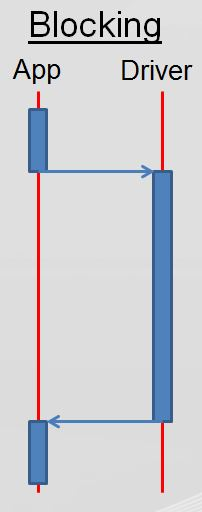
\includegraphics[width=.4\linewidth]{BlockingSequence}
  \caption{Comportamento bloqueante}
  \label{fig:sub1}
\end{subfigure}%
\begin{subfigure}[b]{.5\textwidth}
  \centering
  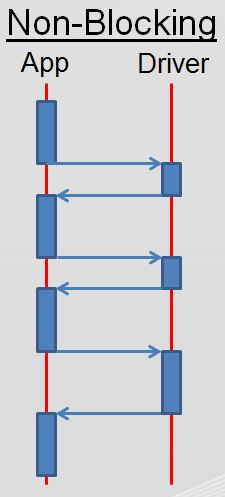
\includegraphics[width=.4\linewidth]{NonBlockingSequence}
  \caption{Comportamento não-bloqueante}
  \label{fig:sub2}
\end{subfigure}
\caption{Comparação entre comportamento bloqueante e não-bloqueante}
\label{fig:test}
\end{figure}

\par A grande maioria dos microcontroladores oferece suporte a interrupções externas. A implementação desse suporte se dá em um pino do microcontrolador que dispara uma interrupção na presença de uma mudança de estado específica no pino. Para que um driver de um dispositivo forneça suporte a interrupções, portanto, basta que o dispositivo possua uma saída que emita uma mudança de estado na ocorrência de eventos relevantes. Ao conectar esta saída ao pino de interrupção externa do microcontrolador, é possível mapear um evento do dispositivo a uma interrupção do microcontrolador, permitindo a orientação a evento que torna possível evitar o bloqueio desnecessário da aplicação.
\par Esse modelo é uma convenção de ambas as partes e se repete nos microcontroladores mais populares do mercado, incluindo Arduino, assim como nos dispositivos externos fabricados para sistemas embarcados. Isso facilita o desenvolvimento de drivers e bibliotecas para ambas as partes.
\par Kits de desenvolvimento para microcontroladores que ajudam a abstrair a implementação do hardware do programador são sempre benéficos por tornarem o processo de desenvolvimento de aplicações para aquele módulo mais simples e acessível. Contudo, os drivers e bibliotecas disponibilizados pela própria Arduino apresentam atualmente funções e módulos que causam o bloqueio da aplicação por utilizarem a técnica de polling, embora existam reimplementações por parte da comunidade de alguns desses módulos de forma a eliminar o bloqueio.

\subsection{Arduino}

\tab Arduino é uma plataforma eletrônica open-source que foca em hardware e software de fácil aprendizado e acesso. Comumente utilizado para prototipação, Arduino conta atualmente com a contribuição de uma vasta comunidade que realiza os mais diversos projetos de sistemas-embarcados, de complexidade variada. \cite{arduinoblog}
\par A plataforma consiste em uma placa de prototipação com um microcontrolador embarcado. A placa possui pinos de entrada e saída com grande foco em GPIO (General Purpose Input and Output). A programação se dá via linguagem C adaptada com bilbiotecas e drivers, com a implementação obrigatória de duas funções que definem a aplicação (ver Exemplo \ref{estruturaarduino}). O conjunto de ferramentas permite a abstração de elementos específicos à programação de microcontroladores como acessos a registradores, por exemplo, permitindo um desenvolvimento mais alto-nível, acessível e portável. Arduino oferece dezenas de placas diferentes, de especificações variadas de forma a atender diversas demandas. A placa mais popular, porém, é a Arduino Uno, que possuiu embarcado o microcontrolador ATmega328P, da Atmel \cite{atmegadatasheet}. Todo o desenvolvimento realizado neste projeto foi focado únicamente na portabilidade para o ambiente deste microcontrolador, embora a adaptação para outros produtos da Arduino seja facilitada pela proposta de portabilidade da empresa.
\begin{lstlisting}[style=CStyle,label=estruturaarduino,caption=Estrutura de uma aplicação Arduino]
void setup(void){
  // Esse bloco é executado uma vez somente, na inicialização da aplicação
}
void loop(void){
  // Este bloco é repetido em loop durante toda o período de execução da aplicação
}
\end{lstlisting}
\par Como já mencionado, microcontroladores Arduino são programados em um ambiente de linguagem C, uma linguagem procedural. A linguagem segue a lógica de procedência temporal e lógica dos comandos por ordem de leitura, o que significa que espera-se que um comando só seja executado quando o precedente acima dele termina sua execução. A utilização da linguagem C para programação em sistemas embarcados, embora bem difundida, sofre com a dificuldade de linguagens procedurais de implementarem a orientação a eventos de forma concisa e clara. Aplicações simples se convertem em pedaços de código de difícil interpretação, como pode ser visto na comparação entre o Exemplo \ref{orientacaoevento1} e \ref{orientacaoevento2}. Nessa comparação possuímos duas implementações que causam o mesmo resultado aparente. O objetivo é que o LED conectado à placa pisque em intervalos de um segundo. O Exemplo \ref{orientacaoevento1} consiste na aplicação feita sem orientação a eventos, o programa acende o LED, aguarda um segundo de forma blocante, desliga o LED e aguarda mais um segundo, repetindo o processo. Já no Exemplo \ref{orientacaoevento2}, a aplicação checa, a toda iteração, o tempo passado. Quando este tempo passa de um segundo, o estado do LED é trocado. Interpretando o código com eventos, a aplicação está aguardando o evento "passou-se um segundo" para então executar o bloco de código "inverta o estado do LED". Embora a lógica seja simples, a implementação nao fica tão clara. Quando aumentamos a complexidade e possuímos mais eventos na aplicação, a legibilidade do código piora mais ainda. 
\begin{lstlisting}[style=CStyle,label=orientacaoevento1,caption=Aplicação não orientada a evento]
/*
  Blink

  Turns an LED on for one second, then off for one second, repeatedly.

  Most Arduinos have an on-board LED you can control. On the UNO, MEGA and ZERO
  it is attached to digital pin 13, on MKR1000 on pin 6. LED_BUILTIN is set to
  the correct LED pin independent of which board is used.
  If you want to know what pin the on-board LED is connected to on your Arduino
  model, check the Technical Specs of your board at:
  https://www.arduino.cc/en/Main/Products

  modified 8 May 2014
  by Scott Fitzgerald
  modified 2 Sep 2016
  by Arturo Guadalupi
  modified 8 Sep 2016
  by Colby Newman

  This example code is in the public domain.

  http://www.arduino.cc/en/Tutorial/Blink
*/

// the setup function runs once when you press reset or power the board
void setup() {
  // initialize digital pin LED_BUILTIN as an output.
  pinMode(LED_BUILTIN, OUTPUT);
}

// the loop function runs over and over again forever
void loop() {
  digitalWrite(LED_BUILTIN, HIGH);   // turn the LED on (HIGH is the voltage level)
  delay(1000);                       // wait for a second
  digitalWrite(LED_BUILTIN, LOW);    // turn the LED off by making the voltage LOW
  delay(1000);                       // wait for a second
}
\end{lstlisting}

\begin{lstlisting}[style=CStyle,label=orientacaoevento2,caption=Aplicação orientada a evento]
/*
  Blink without Delay

  Turns on and off a light emitting diode (LED) connected to a digital pin,
  without using the delay() function. This means that other code can run at the
  same time without being interrupted by the LED code.

  The circuit:
  - Use the onboard LED.
  - Note: Most Arduinos have an on-board LED you can control. On the UNO, MEGA
    and ZERO it is attached to digital pin 13, on MKR1000 on pin 6. LED_BUILTIN
    is set to the correct LED pin independent of which board is used.
    If you want to know what pin the on-board LED is connected to on your
    Arduino model, check the Technical Specs of your board at:
    https://www.arduino.cc/en/Main/Products

  created 2005
  by David A. Mellis
  modified 8 Feb 2010
  by Paul Stoffregen
  modified 11 Nov 2013
  by Scott Fitzgerald
  modified 9 Jan 2017
  by Arturo Guadalupi

  This example code is in the public domain.

  http://www.arduino.cc/en/Tutorial/BlinkWithoutDelay
*/

// constants won't change. Used here to set a pin number:
const int ledPin =  LED_BUILTIN;// the number of the LED pin

// Variables will change:
int ledState = LOW;             // ledState used to set the LED

// Generally, you should use "unsigned long" for variables that hold time
// The value will quickly become too large for an int to store
unsigned long previousMillis = 0;        // will store last time LED was updated

// constants won't change:
const long interval = 1000;           // interval at which to blink (milliseconds)

void setup() {
  // set the digital pin as output:
  pinMode(ledPin, OUTPUT);
}

void loop() {
  // here is where you'd put code that needs to be running all the time.

  // check to see if it's time to blink the LED; that is, if the difference
  // between the current time and last time you blinked the LED is bigger than
  // the interval at which you want to blink the LED.
  unsigned long currentMillis = millis();

  if (currentMillis - previousMillis >= interval) {
    // save the last time you blinked the LED
    previousMillis = currentMillis;

    // if the LED is off turn it on and vice-versa:
    if (ledState == LOW) {
      ledState = HIGH;
    } else {
      ledState = LOW;
    }

    // set the LED with the ledState of the variable:
    digitalWrite(ledPin, ledState);
  }
}
\end{lstlisting}
\par De um ponto de vista mais funcional, o código também desperdiça ciclos computacionais pelo volume de verificações. O evento é verificado frequentemente para que o sistema permaneça responsivo, sacrificando ciclos pelas verificações que falham, em um exemplo de polling. Outro problema causado por este modelo é que, no caso de um sistema mais complexo, manter a responsividade se torna inviável, já que o bloco iterado pela aplicação cresce e os intervalos entre verificações de cada evento crescem. O uso de interrupções faz um bom papel de amenizar a questão da responsividade. No Exemplo \ref{interrupcao1} possuímos um código que atinge o mesmo resultado dos Exemplos \ref{orientacaoevento1} e \ref{orientacaoevento2}, porém fazendo o uso de interrupções. A aplicação faz uso de um timer interno ao microcontrolador para gerar uma interrupção a cada um segundo. Cada vez que a interrupção ocorre, a aplicação executa um bloco de código associado à interrupção, uma função de callback. Essa função configura o valor de uma variável que marca o acontecimento do evento. No bloco principal da aplicação, o valor desta variável é checado para se detectar o acontecimento do evento e realizar a ação correspondente, que neste caso é inverter o valor do LED.
\par Neste exemplo o sistema fica mais responsivo pois o bloco principal só consulta o valor da variável. O problema de desperdício de ciclos permanece, porém, já que a consulta à variável permanece, caracterizando polling novamente. O código também não é claro já que o entendimento depende da compreensão da interrupção e de como as duas sessões do código (callback da interrupção e consulta no bloco principal) interagem.

\begin{lstlisting}[style=CStyle,label=interrupcao1,caption=Aplicação utilizando interrupção]
#define ledPin 13
volatile bool timerEvent = FALSE;
void setup()
{
 pinMode(ledPin, OUTPUT);

 // initialize timer1 
 noInterrupts();    // disable all interrupts
 TCCR1A = 0;
 TCCR1B = 0;

 TCNT1 = 3036;    // preload timer 65536-16MHz/256/1Hz
 TCCR1B |= (1 << CS12);    // 256 prescaler 
 TIMSK1 |= (1 << TOIE1);   // enable timer overflow interrupt
 interrupts();    // enable all interrupts
  
 Serial.begin(9600);
}

ISR(TIMER1_OVF_vect)
{
 timerEvent = TRUE;
}

void loop()
{
 if(timerEvent){
  timerEvent = FALSE;
  digitalWrite(ledPin, digitalRead(ledPin)^1);
 }
}
\end{lstlisting}
\subsection{Céu}
\tab Céu é uma linguagem síncrona reativa estruturada desenvolvida na PUC-Rio. A semântica de Céu permite ao usuário escrever uma aplicação reativa orientada a eventos contendo paralelismo e concorrência de forma determinística e clara. A compilação de um programa em Céu consiste na transcrição do código para seu equivalente em C para então ser compilado no compilador C de escolha, gerando o executável final. Devido à portabilidade de código C, Céu se prova uma linguagem portável e de variável uso. Apesar disso, a linguagem se destaca em aplicações que envolvem coordenação com eventos externos, como GUIs, jogos e, mais relevante para este trabalho, sistemas embarcados.
\par Falar aqui sobre o paralelismo de Céu, explicando trails e o determinismo.

\par O foco da linguagem na orientação a eventos se dá pelas diretivas naturais de aguardar um evento ("await") e emitir um evento ("emit"). Um fluxo de execução de uma aplicação em Céu   
\subsection{Céu-Arduino}

\par O kit de desenvolvimento Céu-Arduino apresenta uma abordagem única para o desenvolvimento
orientado a eventos e suporte a interrupções, e se encontra atualmente em um estado inicial. O
projeto está em uma versão 0.20 e conta com exemplos básicos de aplicações em Arduino queutilizam a linguagem Céu. Apesar de não possuir somente poucas bibliotecas e drivers desenvolvidos
em Céu, a linguagem é de fácil integração com C, sendo possível utilizar os módulos desenvolvidos
atualmente para Arduino. \cite{githubceuarduino}

\section{Drivers}

\subsection{Metodologia}
\subsubsection{Estudo do Ambiente}
\paragraph{Estudo do Ambiente de Desenvolvimento C}
\paragraph{Estudo do Hardware}
\subsubsection{Implementação Intermediária}
\paragraph{Implementação Original}
\paragraph{Implementação Mínima Viável}
\subsubsection{Implementação Final}
\paragraph{Estudo do Ambiente de Desenvolvimento Céu}
\paragraph{Implementação em Céu}


\subsection{Analog I/O}

\tab Como primeira etapa do projeto foram definidos os módulos para os quais implementações não-
bloqueantes em Céu serão desenvolvidas. Os módulos são Entrada e Saída Analógica (Analog
I/O), Comunicação SPI (SPI), Comunicação Serial (Serial), Suporte a RTC Externo
(External RTC) e Operações na EEPROM (EEPROM). Os módulos foram descritos na ordem
estimada de dificuldade crescente.
\par O realizado dentro desta primeira etapa do projeto girou em torno do desenvolvimento de um dos
módulos. Para que o driver fosse implementado, foi necessário um estudo não só da plataforma
Arduino e do microcontrolador, mas também do ambiente de desenvolvimento disponibilizado pela
AVR e das bibliotecas já implementadas e disponibilizadas em Céu, principalmente as de Céu-
Arduino.
\par Todo o código desenvolvido neste projeto segue a intenção de priorizar simplicidade e rapidez na
execução, respeitando os requisitos de um módulo suficientemente robusto e funcional. De tal
modo, os drivers desenvolvidos atenderão somente a plataforma Arduino Uno, por ser a mais
utilizada e disponível, além de possuírem limitações que podem vir a exigir atenção e
responsabilidade do usuário final no uso dos drivers em aplicações. O motivo é a busca por uma
melhor utilização do tempo do projeto e redução da carga computacional para a execução dos drivers.
\par Ao final desta etapa, o projeto se encontra com um driver já desenvolvido e em uma versão estável.
Tal módulo servirá como base para que o processo de desenvolvimento possa ser reproduzido para
os demais drivers. A explicação de cada etapa nesta sessão do relatório virá acompanhada do exemplo
prático da implementação referente ao módulo. Deste modo, o processo será descrito assim como o
desenvolvimento do driver.
\par O módulo desenvolvido nesta primeira etapa do projeto é o de leitura e emissão de valores de
voltagem analógicos. A referência para este módulo no texto daqui em diante será “Analog I/O”,
significando “Entrada e Saída Analógica”.

\paragraph{Estudo do Ambiente}

\tab O ambiente de desenvolvimento que usa a linguagem C é o mesmo tanto para Arduino quanto para
Céu-Arduino. Isto é, ambos os códigos são em alguma etapa compilados utilizando o mesmo
compilador. Esse compilador é disponibilizado pela AVR e é uma versão customizada de GCC,
chamada de AVR-GCC. Em conjunto com o compilador, são utilizadas bibliotecas da AVR que
tratam da abstração do hardware, como acesso a registradores, para variados chips da Atmel, incluindo
o AtMega328p, presente no Arduino Uno, plataforma para qual os módulos deste projeto são
destinados.
\par Outra ferramenta essencial para o andamento do projeto é a capacidade de se registrar rotinas de
serviço a interrupções (Interrupt Service Routines, ISR), que são rotinas de código associadas a
interrupções do microcontrolador. Em outras palavras, quando o hardware emite uma interrupção, osoftware executaria a ISR atrelada àquela interrupção. AVR disponibiliza uma biblioteca de tratamento
de interrupções que torna simples a implementação de tais ISRs.
\par Para Analog I/O, isso significa que teremos fácil acesso a quaisquer registradores atrelados ao
módulo, e o acesso ao hardware ficará transparente para o desenvolvedor, que irá tratar os
registradores como vetores de bits. Como será mencionado posteriormente, isso procede tanto para
o ambiente de desenvolvimento C quanto o ambiente Céu.
\par AVR disponibiliza um documento detalhado \cite{wortmann2015} das especificações do microcontrolador presente no
Arduino Uno, o AtMega328p. Esse documento, chamado datasheet, possui a definição de todas as
funcionalidades e hardwares dedicados presentes, incluindo a definição e descrição dos registradores
responsáveis e atrelados a cada um. Esse documento é vital para o entendimento das capacidades e
limitações do chip e, principalmente, o de como operá-lo.
\par A datasheet está no centro da primeira etapa do desenvolvimento, que é estudar o funcionamento do
hardware para que, em conjunto com o estudo do código da implementação atual (se existente), seja
possível compreender o comportamento de uma API tradicional. O foco desse passo é criar uma
base de conhecimento sobre as informações já disponíveis acerca do módulo.
\par Durante essa etapa no desenvolvimento do Analog I/O, foi levantado que as funcionalidades de
entrada (leitura de valor analógico) e saída (emissão de valor analógico) são atreladas a hardwares
dedicados distintos no microcontrolador. Enquanto os valores de saída analógicos são simulados
utilizando ondas PWM (o pino liga e desliga em intervalos regulares, onde o valor analógico seria a
razão entre o tempo que permanece ligado e o tempo que permanece desligado). Essa funcionalidade
já se encontra implementada em Céu e, portanto, não é pertinente para os efeitos deste relatório.
\par Os valores de leitura, em outra mão, são obtidos por um hardware de Conversão Analógica para
Digital (ADC). Esse componente dedicado recebe um valor de voltagem analógico e, após ciclos de
processamento, guarda em seus registradores a representação de 10 bits deste valor, quando
comparado a uma referência de valor máximo. Em outras palavras, se a voltagem de entrada for o
ground, o resultado será “0”. Caso seja igual ou acima da voltagem de referência, será 1023.
\par Embora existam mais de um pino de leitura analógico no microcontrolador, existe somente um
hardware de ADC. Para que possa atender a todos os seis pinos, o hardware conta com um
multiplexador que seleciona o pino para qual a leitura deve ser feita. Repare que não é possível ter
mais de um pino tendo seu valor lido pelo hardware ao mesmo tempo. O valor desse multiplexador se
encontra em um dos registradores ao qual o desenvolvedor possui acesso e, portanto, seu valor pode
ser modificado facilmente. Além do multiplexador, o usuário possui acesso a vários valores que
servem como configuração do ADC. Dentre esses valores, o de Analog to Digital Interrupt
Enable (ADIE) é de elevado interesse ao projeto, já que quando este bit, presente no registrador de
configuração ADCSRA, se encontra “setado” (valor lógico 1), o hardware dispara uma interrupção
toda vez que uma conversão termina.
\par Em resumo, para efetuar uma conversão, o multiplexador, cujo valor é controlado pelo registrador
ADMUX, deve receber o valor do pino para qual a leitura será feita. Do mesmo modo, os outros
bits de configuração devem ser setados de acordo com a configuração desejada pelo usuário. Para
iniciar a conversão, basta que o software escreva o valor lógico 1 no bit ADSC. Esse bit terá seu valor
1 mantido pelo hardware enquanto a conversão está em progresso, e será zerado no momento que a
conversão tiver fim e o resultado estiver disponível. Os nomes técnicos dos bits e registradores serão
referenciados no texto quando descrevendo a implementação.

\paragraph{Implementação Intermediária}

\tab A implementação atual de uma função de leitura analógica, presente na biblioteca de funções
disponibilizada pela Arduino, possui como único argumento o pino para qual a conversão deve ser
feita, devolvendo o resultado da mesma.
\par A função configura os registradores do hardware, incluindo ADMUX, cujo valor terá como base o
argumento de entrada da função. Em seguida, inicia a conversão escrevendo o lógico 1 em ADSC.
Para aguardar o fim da conversão, o código faz polling em ADSC. Como já discutido, isso caracteriza
o motivo da aplicação apresentar um comportamento bloqueante, e é o que o projeto visa eliminar.
Após ADSC ter sido zerado pelo hardware, a função segue sua execução e retorna o valor do
resultado.
\par Após a funcionalidade ter sido estudada do ponto de vista do hardware e do software (caso este seja
disponível), a causa do comportamento bloqueante da aplicação deverá ter sido identificada e uma
solução idealizada. Essa solução pode ter como base a capacidade do hardware de gerar interrupções
ou quaisquer outros métodos para que não seja necessário à aplicação consultar o hardware, e sim
cadastrar um call-back para que o modelo de Céu funcione.
\par Com base na solução, deverá ser implementada uma API na linguagem de escolha. No âmbito deste
projeto, essa linguagem será C. Embora possa não se assemelhar com a implementação final, essa
solução intermediária deve apresentar contribuições claras ao código final, mesmo que na forma de
aprendizado.
\par A implementação em C do driver para gerenciar o ADC buscou eliminar o polling encontrado (descrito
na última sessão) utilizando a capacidade do módulo de emitir uma interrupção quando a conversão
for concluída e o registro de uma ISR atrelada a essa interrupção utilizando as utilidades
disponibilizadas pela AVR.
\par A implementação nova reaproveita a implementação original, modificando a lógica do polling.
Enquanto a original possuía apenas uma função que encapsulava todo o processo de leitura, desde a
configuração do hardware dedicado até o retorno do valor, a API nova é dividida em três funções, que
contam com o suporte de uma ISR atrelada à interrupção do ADC e uma variável global que guarda
o estado de uma conversão.
\par A primeira função é equivalente à função de leitura da implementação original até o momento do
início da conversão, isto é, ela termina quando ADSC recebe o valor lógico 1. Entretanto ela
configura ADIE para que as interrupções ocorram, algo que não estava previsto na implementação
da Arduino. Essa função altera o valor da variável de estado para que esta reflita que uma conversão
está em andamento.
\par A segunda função é utilizada para consultar a variável de estado de modo a saber se uma conversão
está acontecendo. Isso é necessário pois caso esteja, os valores contidos nos registradores que
guardam o resultado da conversão podem não ser verdadeiros.
\par A terceira função é equivalente à parte final da função da implementação original, após o polling. Ela
simplesmente retorna o resultado da conversão contido nos registradores.
\par A ISR atrelada à interrupção do ADC altera o valor da variável de estado para refletir que uma
interrupção terminou.
\par Para efetuar uma leitura de um valor analógico utilizando esta API, o usuário deve chamar a primeira
função para iniciar a conversão e, depois que a segunda função retorne um valor negativo
(representando que uma conversão não está em progresso), chamar a terceira função para obter o
resultado.

\paragraph{Implementação Final}

\tab A linguagem Céu permite uma forte integração com C, sendo capaz de chamar funções e acessar
variáveis declaradas e contidas no contexto C. Isso permite que parte da implementação mínima
viável seja reutilizado no desenvolvimento da versão da API em Céu. O ambiente também permite a
declaração de ISRs, o que torna possível reproduzir a API em C dentro do ambiente Céu desde o
primeiro momento.
\par A vantagem de Céu é a modelagem orientada a eventos, o que permite que a API execute baseada
em call-backs, contribuindo para a eliminação do desperdício dos ciclos (que eram utilizados para
checar se a API e encontrava em um estado que permitia a próxima ação). Este passo no
desenvolvimento deve ser utilizado para modelar a solução concebida nos passos anteriores de forma
que utilize as vantagens de Céu a favor da economia de ciclos, implementando a estrutura de
orientação a eventos prevista no modelo Céu.
\par Nesta etapa do desenvolvimento do módulo ADC, a obtenção do resultado da conversão foi
modelada como um evento emitido pelo driver. Deste modo, a API consiste na requisição de uma
conversão por parte da aplicação e da emissão, por parte da API, de um evento que carrega o
resultado.
\par Após ter a API modelada em Céu, o desenvolvedor possuiu todas as ferramentas para produzir a
solução final. Deve-se buscar tirar o máximo de proveito possível do trabalho realizado nas etapas
anteriores.
\par A implementação em Céu do módulo ADC constituiu ter uma função que iniciava uma conversão,
função esta que foi reaproveitada da API em C. Como a própria API será responsável por emitir o
resultado quando a conversão terminar, não há necessidade de manter uma variável de estado. Basta
que, na ISR, o resultado seja obtido utilizando a função implementada no passo anterior e que este
valor seja enviado à aplicação na forma de um evento. Todo o controle de estados do driver é
encapsulado pelo próprio modelo de Céu e o fluxo de execução.
\par Para efetuar uma conversão, a aplicação, agora em Céu, deve requisitar uma conversão e “aguardar”
o evento resultado. Como previsto no ambiente Céu, enquanto a aplicação está “aguardando” o
evento, o microcontrolador fica livre para executar outras linhas de código pendentes ou, caso
nenhuma exista, entrar em um estado de baixo consumo de energia. Quando o hardware concluir a
conversão, o evento emitido irá “acordar” a aplicação, que seguirá seu fluxo. No caso da
implementação original, a aplicação não poderia fazer uso desse tempo de “aguarde” pois estaria
bloqueada consultando o driver para saber se a conversão já havia terminado. O contraste entre as
duas aplicações e, por consequência, o contraste entre as duas APIs ficam claros.

\subsection{SPI}

\paragraph{Estudo do Ambiente}
\paragraph{Implementação Intermediária}
\paragraph{Implementação Final}

\subsection{RF24}

\paragraph{Estudo do Ambiente}
\paragraph{Implementação Intermediária}
\paragraph{Implementação Final}

\section{Aplicação}

\subsection{Proposta}
\subsection{Desenvolvimento}
\subsection{Resultado}

\section{Comentários Finais}

\newpage

\printbibliography

\end{document}
